\documentclass[sigconf]{acmart}
\settopmatter{printacmref=false} % Removes citation information below abstract
\renewcommand\footnotetextcopyrightpermission[1]{} % removes footnote with conference information in first column
\pagestyle{plain} % removes running headers
\setcopyright{none}

\usepackage{booktabs} % For formal tables
\usepackage[ruled]{algorithm2e} % For algorithms
\renewcommand{\algorithmcfname}{ALGORITHM}
\SetAlFnt{\small}
\SetAlCapFnt{\small}
\SetAlCapNameFnt{\small}
\SetAlCapHSkip{0pt}
\IncMargin{-\parindent}

\usepackage[latin1]{inputenc}
\usepackage{graphicx}
\usepackage{amsmath}
\usepackage{amsfonts}

\DeclareMathOperator*{\argmax}{argmax}

\begin{document}

\title{Named Entity Recognition on HTML as an information extraction subtask}

\author{Jo�o Mateus de Freitas Veneroso}
\affiliation{%
  \institution{Universidade Federal de Minas Gerais}
  \streetaddress{Av. Pres. Ant�nio Carlos, 6627 - Pampulha}
  \city{Belo Horizonte}
  \state{MG}
  \postcode{31270-901}
  \country{Brazil}}
\email{jmfveneroso@gmail.com}

\author{Berthier Ribeiro-Neto}
\affiliation{%
  \institution{Universidade Federal de Minas Gerais}
  \streetaddress{Av. Pres. Ant�nio Carlos, 6627 - Pampulha}
  \city{Belo Horizonte}
  \state{MG}
  \postcode{31270-901}
  \country{Brazil}}
\email{berthier.dcc.ufmg@gmail.com}

\begin{abstract}

Reliable researcher affiliation data is necessary to allow enquiring
about international research group productivity and publication patterns.
Public bibliographic databases such as DBLP and Google Scholar hold
invaluable data about the academic environment. However, the researcher
affiliation information is frequently missing or outdated.
We propose a statistical data extraction method to acquire affiliation 
information directly from university websites and solve the name extraction
task in general.
Previous approaches to web data extraction either lack in flexibility,
because wrappers do not generalize well on cross website tasks, or 
they lack in precision, because domain agnostic methods neglect 
useful properties of this particular application domain.
Our statistical approach solves the name extraction task with 
a framework that incorporates both textual and structural features to
yield an outstanding tradeoff between generality and precision. 
We conducted experiments over a collection of 152 faculty 
web pages in multiple languages from universities in 49 countries
and obtained 94.40\% precision, 97.61\% recall and 0.9597 F-measure at
the extraction task.


\end{abstract}

% \keywords{Named entity recognition, information extraction, web data extraction}

\maketitle

% ==========================================
% Beginning of text.                       |
% ==========================================

\section{Introduction}

Web information extraction is the task of automatically extracting structured information
from unstructured or semi-structured web documents. The input usually consists of
web documents containing a number of predetermined entities organized in a similar 
manner and the information extraction task consists of identifying these entities
and organizing them according to a template. In this context, named entity recognition
(NER) is a subtask that aims to detect named entities in the text and classify them into 
predetermined categories such as person names, locations or organizations. Once we are able
to reliably detect the relevant entities, we may employ an information extraction 
algorithm to extract structured data. In this paper, we investigate different NER 
approaches from the perspective of web information extraction.

HTML documents most often lie in between the structured / unstructured data paradigm, 
which means that authors take quite a casual approach regarding formal structure. 
However, DOM hierarchy, element disposition, class names, and other features related to 
the document structure and indirectly associated with the data itself can be valuable 
information in the task of identifying entities and determining relationships. Yet we 
cannot expect these features to be completely constrained by an underlying pattern. 
Organization patterns tend to follow some guidelines but are in no way subject to 
strict rules. That is why classical information extraction systems such as automatic
wrapper generators usually do not translate well across different websites. Contrastingly, 
statistical based approaches can be much more flexible.

NER systems are frequently trained and tested on news corpora such as the 
dataset introduced at the Language-Independent Named Entity Recognition Shared Task
at CONLL-2003 \cite{Sang2003}. State-of-the-art approaches have recently achieved 
F1-scores of 90.10 \cite{Huang2015}, 90.94 \cite{Lample2016}, and 91.21 \cite{Ma2016} 
in this task using different combinations of bidirectional LSTM layers, word and 
character representations. 

NER on HTML poses a different type of challenge, because web pages are often
very different from the plain text found in news corpora. Named entities may be present 
inside tables, lists, graphs or other types of visual elements that provide
little to no contextual information that could give hints about the semantic category of 
a word. Systems trained on news or similar corpora do not translate well to the web
NER task without requiring some sort of retraining, since in this task we cannot profit
as much from contextual hints or transfer learning approaches such as word embeddings.
Besides, deep learning approaches can require a lot of data to reach peak performance. 
Therefore, in cases where there is little labeled data, we find that generative approaches 
may work better.

To test different NER approaches from the perspective of web information extraction,
we will explore the task of person names extraction from university faculty websites.
Researcher affiliation is often missing from many entries in public databases such as DBLP  
\footnote{
  http://dblp.uni-trier.de/
} and the display of information varies significantly between different university 
websites, so this task can provide a good measure of the expected performance and
data need for other web information extraction tasks. Also, with the lack of a large amount
of training data, we show that feature engineering and resources such as a gazetteer 
may be invaluable.

% \begin{figure}
%   \centering
%   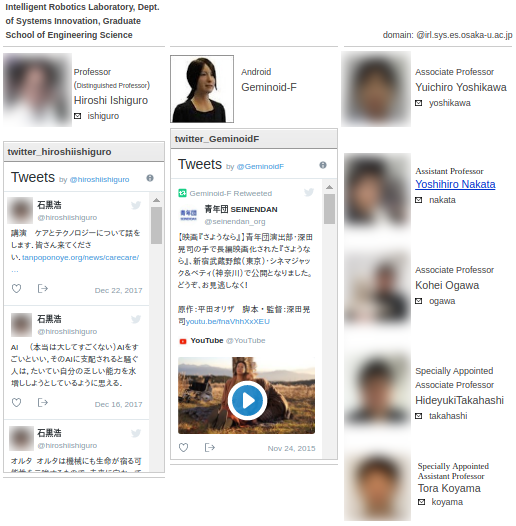
\includegraphics[width=0.5\textwidth]{pics/jap_osaka_lab}
%   \caption{Example of a faculty directory}
%   \label{fig:faculty_directory}
% \end{figure}
% 
% To acknowledge the complexity of this extraction task, take for example a snippet of 
% the staff page for the intelligent robotics laboratory from Osaka University shown in figure 
% \ref{fig:faculty_directory}. There is some structure to the way member profiles are arranged, 
% but the organization is rather flexible, also note that there is little text to contextualize
% each named entity. 

\section{Related Work}

In the last 20 years, the astonishing growth of public information in the web has 
led to the development of a number of different approaches to the problem of web 
information extraction. Traditionally, the task was solved by designing special purpose
programs called wrappers to recognize relevant data and store records in a structured
format. These early tools varied wildly relative to their degree of automation. 

It was readily perceived that manual wrapper generation was a rather tedious and
error prone process, unsuited for large scale operations. Wrappers tend to
break frequently because they rely heavily on web page features that can change 
often. So, in the late nineties, several authors advocated for wrapper induction, a technique 
that consists of automatically constructing wrappers from a small set of examples by 
identifying delimiters or context tokens that single out the desired attributes. 
Some remarkable wrapper induction methods are WIEN \cite{Kushmerick2000}, Soft 
Mealy \cite{Hsu1998} and STALKER \cite{Muslea1999}.

Despite being better than constructing wrappers manually, wrapper induction methods 
still suffered from a lack of expressive power and flexibility. These methods had 
trouble handling records with missing attributes or unusual structures because
patterns could only be identified if they happened at least once in the examples.

Other approaches such as NoDoSE (\cite{Adelberg1998}) and Debye (\cite{Laender2002a}) 
brought greater flexibility to wrapper induction methods by requiring a greater level 
of human interaction through graphical user interfaces. Web data extraction techniques often 
require some sort of assistance from human experts to boost accuracy. One of the main challenges 
in the field lies in determining an adequate tradeoff between the degree of automation and 
the precision and recall of the data extraction tool.

To automate the task of web data extraction completely some approaches,
such as Road Runner \cite{Crescenzi2001}, removed entirely the need for data examples.
Road Runner parses documents belonging to a same class (e.g. books on Amazon) and 
generates wrappers based on their similarities and differences, yielding comparable results 
to those obtained by wrapper induction methods. However like previous approaches, it was 
unsuited for cross site extraction tasks because the learned rules were not general enough.

NLP based approaches aimed at extracting more general rules that could possibly
be employed over multiple websites. RAPIER \cite{Califf1999} is a method of rule
extraction that uses information such as part-of-speech tags and semantic classes from
a lexicon to derive patterns from a set of training examples. This approach is more
flexible than the wrapper induction methods, however it achieves much lower rates of 
recall and precision.

In 2002, a survey by Laender et al. \cite{Laender2002} made a thorough classification of the
early approaches with a taxonomy based on their main technology, being them: languages for
wrapper development, HTML-aware tools, NLP-based tools, Wrapper Induction Tools,
Modeling-based tools and Ontology-based tools. Some noteworthy examples from this era
are: 

\begin{itemize}
\item TSIMMIS \cite{Hammer1997} and WebOQL \cite{Arocena1999}, which are special purpose 
languages for building wrappers.

\item Road Runner \cite{Crescenzi2001}, XWRAP \cite{Liu2000} and W4F \cite{Sahuguet1999}, 
which are HTML-aware tools that infer meaningful patterns from the HTML structure.

\item RAPIER \cite{Califf1999}, SRV \cite{Freitag1998}, WHISK \cite{Soderland1999}, which 
are NLP-based tools.

\item WIEN \cite{Kushmerick2000}, Soft Mealy \cite{Hsu1998} and STALKER \cite{Muslea1999} which 
are wrapper induction methods.

\item NoDoSE \cite{Adelberg1998} and Debye \cite{Laender2002a}, which are semi supervised modeling
based tools that require some interaction with the user by means of a graphical
user interface.
\end{itemize}

In 2006, Chang et al. \cite{Chang2006} complemented the previous surveys with semisupervised 
technologies such as Thresher \cite{Hogue2005}, IEPAD \cite{Chang2001} and 
OLERA \cite{Chang2004}. They differed from supervised 
and unsupervised methods because they either needed only a rough description of
data from users for extraction rule generation or some level of post processing
that needed user attention. The survey also mentioned newer unsupervised methods
such as DeLa \cite{Wang2003}, Exalg \cite{Arasu2003} and Depta \cite{Zhai2005}.

Most of the early information extraction systems were rule-based with either 
manual rule description or automatic rule learning from examples, thus they
suffered from a lack of flexibility when dealing with noisy and unstructured data.
Huge progress in the field of statistical learning led to the development of
statistical models that tried to solve this problem.

In 2008, Sarawagi \cite{Sarawagi2008} produced a survey that classified wrappers in
rule-based methods, statistical methods and hybrid models, bringing together 
the fields of named entity recognition, relationship 
extraction and information extraction. The rule based methods encompass most of the 
previous models. The statistical methods convert the extraction task into a token labeling 
task, identifying the target entities through the assignment of labels as in a typical 
Named Entity Recognition task. Traditionally, Hidden Markov Models, Linear Chain Conditional 
Random Fields \cite{Lafferty2001}, and Maximum Entropy Taggers have been the usual choice 
for linear sequence tagging models.

More recently, with the advancement in Natural Language Processing and Deep Learning, 
neural models outperformed previous NER methods. Using a bidirectional Long Short-Term
Memory (LSTM) model with a Conditional Random Field (CRF) output layer, \cite{Huang2015} 
obtained 90.10 F1 score on the CoNLL 2003 corpus for named entity recognition. A similar model
by \cite{Lample2016} incorporates a Convolutional Neural Network over character embeddings
as an input to the bidirectional LSTM reaching an F-score of 90.94 at the same task. Finally, 
\cite{Ma2016} constructed word representations with the hidden layer of a bidirectional 
LSTM obtaining an F-score of 91.21. The latter two models make use of orthographic and 
morphological evidence to detect named entities, making the models less reliant on feature
engineering and surrounding words. Up to our knowledge, these models still have not been
employed at the web information extraction task.

Surveys by Ferrara et al. \cite{Ferrara2014} and Schulz et al. \cite{Schulz2016} 
updated the previous surveys on information extraction methods with some interesting innovations. 
Some examples are: the Visual Box Model \cite{Krupl2005}, a data extraction system that produces 
a visualization of the web page to exploit visual cues to identify data presented in a tabular form;
automatic wrapper adaptation \cite{Ferrara2011}, a technique that tries to reduce the cost of 
wrapper maintenance by measuring the similarity of HTML trees and adapting
wrappers to the new page structure; AutoRM \cite{Shi2015}, a method to mine
records from a single web page by identifying similar data regions through DOM
tree analysis; and Knowledge Vault \cite{Dong2014}, a method that combines different 
extraction approaches to feed a probabilistic knowledge base.

In 2016, Varlamov et al. \cite{Varlamov2016} argued that the degree of automation can no
longer be the main classification criterion for the data extraction systems
because unsupervised methods which were widely considered to be the state 
of the art when dealing with individual websites performed poorly or were
innapropriate on cross site extraction tasks. The authors proposed a 
classification of methods by the extent of their application. 
The competing approaches were separated into two groups: methods for individual 
websites and methods that are applicable to whole application domains. 

The first group contains most of the earlier approaches, including the supervised
approaches: SRV \cite{Freitag1998}, RAPIER \cite{Califf1999}, WHISK \cite{Soderland1999}, 
WIEN \cite{Kushmerick2000} SoftMealy \cite{Hsu1998} and STALKER \cite{Muslea1999}; and
the unsupervised approaches: RoadRunner \cite{Crescenzi2001} and EXALG \cite{Arasu2003}.

The second group is divided between domain specific methods and domain agnostic methods.
Domain specific methods are designed for extracting data about a particular 
application domain across multiple websites.
Domain specific methods integrate information about the particular application domain in the 
course of its development and thus are able to achieve superior performance in
comparison to domain agnostic methods. One example is the method of comment extraction 
from blog posts described by Kao et al. \cite{Kao2010}. 

Domain agnostic methods are the most general extraction methods. They can extract
information from any application domain from multiple websites. They pose the hardest
challenge because the tool must infer data relevance without any prior training in
that particular application domain. Some examples are: ODE (\cite{Su2009}), ObjectRunner 
(\cite{Abdessalem2010}), and AMBER (\cite{Furche2012}). These approaches are more flexible but 
yield worse results than domain specific methods.

In this paper, we are exploring NLP based approaches to solve a domain specific problem.


\section{NER Models}

We explored multiple approaches to the Named Entity Recognition problem in the context 
of a web information extraction task. 

\subsection{Hidden Markov Model}

A Markov Model is a stochastic model that computes the most probable
sequence of states given a set of observable states $ \S = \{s_1, s_2, ..., s_n \} $.
The Hidden Markov Model (HMM) differs from the Markov Model in that it
does not observe the states directly, but rather a probabilistic function of those 
states. For example in NER, the words are observed, however the Named Entity labels
associated with these words are not. Formally, we want to compute the most probable
sequence of labels $ Y = {y_1, y_2, ..., y_n} $ for a sequence of observed tokens
$ X = {x_1, x_2, ..., x_n} $.

\[

Y = argmax P(Y|X)

\]

Using Bayes theorem:

\[

P(Y|X) = \frac{P(X|Y) P(Y)}{P(X)}

\]

Since $ P(X) $ is the same for all labels sequences, we can simply maximize:

\[

Y = P(X|Y) P(Y)

\]

A Hidden Markov tagger makes two assumptions. First, the 
probability of being in a given state depends only on a fixed number of previous states.
That is $ P(y_i|y_{i-1}x_{i-1}, y_{i-2}x_{i-2}, ..., y_1x_1) = P(y_i|y_{i-1}, y_{i-2},..., y_{i-k}) $. In fact, 
we can get much better results at the NER on HTML task by looking at trigrams
or quadrigrams instead of bigrams as in a regular Markov Model. Some 
label assignments are highly improbable, such as single token named entities separated 
by an Other label, and these kinds of patterns can be caught by a higher order Hidden
Markov Model. Second, the probability of a word depends only on its assigned label 
$ P(x_i|y_{i-1}x_{i-1}, ..., y_1x_1) = P(x_i|y_i) $. Finally, the probability 
$ P(Y|X) $ can be computed with the expression:

\[

P(Y|X) = \prod P(y_i|y_{i-1}, y_{i-2}, ..., y_{i-k}) P(x_i|y_i)

\]

The probabilities can be calculated via maximum likelihood estimation from the relative
frequency of labels and words in the corpus. The best sequence of labels can be computed 
with the Viterbi algorithm. However,
as we increase the order of the Markov Model ($k$ in Equation 1) this computation becomes 
exponentially more expensive. The beam-search strategy may be employed for a faster search,
but we found that for $ k \leq 3 $, the Viterbi algorithm is still viable.

Hidden Markov Models taggers have been succesfully apllied in many NLP tasks and they are 
incredibly fast to train, making them a good choice for a first approximation. However, these
models are highly dependent on the right selections of features, what may outweigh the 
benefit of a small training cost.

\subsubsection{Self training}

\subsection{Linear Chain Conditional Random Fields}

A Linear Chain Conditional Random Field (CRF) is the discriminative analog to the HMM.
It is a distribution $ P(Y|X) $ that takes the form:

\[

P(Y|X) = \frac{1}{Z(x)}\prod exp \left{ \sum_{k=1}^{K} \theta_k f_k(y_{t-1}, y_t, x_t) \right}

\]

where $ \theta $ is the parameter vector that we are going to learn, $ f_k(y_{t-1}, y_{t}, x_t) $ 
is a feature function over the current and previous timesteps and the current word $ x_t $, and
$ Z(x) $ is a partition function that depends on the input. Linear chain conditional random fields
are more general than Hidden Markov Models because the transition from $ y_{t-1} $ to $ y_{t} $ can
depend on the current observation $ x_t $. In fact, linear chain CRFs do not assume independence 
between the input variables $ x $. 

Linear Chain CRFs are a natural fit to Named Entity Recognition problems because of the
high label dependency. Therefore, sequence taggers that do not take this output dependency into
account tend to perform poorly. More recently, CRFs have been employed as the output layer
in neural models to account for the label dependency, producing significant improvement over
models that output labels independently.

Label sequences can be decoded with the Viterbi algorithm like HMMs.

\subsection{Neural Models}

Recurrent neural networks (RNN) have been succesfully employed on numerous NLP tasks such as
language modelling, POS tagging, speech recognition and NER. Different
from feedforward neural networks, RNNs can retain information in their internal state,
making them more suitable for processing sequences, and consequently for solving text related
tasks. In NER, the network outputs one label for each input vector. Although RNNs are theoretically 
capable of learning long term dependencies, in practice 
it might be difficult, as shown by \cite{Hochreiter1991}. Long short term memory networks
(LSTM) were introduced \cite{Hochreiter1997} with this problem in mind and have been popularized
since them. The LSTM cell has has the following definition:

\[
\Gamma_f = \sigma(W_f[a])
\]

\[
\]

In NER related tasks, both past and future input features are important when deciding the
label at time $ t $, thus we may employ a bidirectional LSTM (Graves et al., 2013). to 
account for this fact. Bidirectional LSTMs are simply two separate LSTM networks where
the first one receives the backward states and the second is fed in reverse order 
with the forward states XXXX. The hidden layers of both networks are combined and fed to 
the output layer.

\cite{Huang2015} proposed a bidirectional LSTM with a CRF layer (LSTM-CRF) on the output to tackle
the sequence tagging problem. The CRF layer jointly decodes labels for the whole sentence instead
of predicting each label individually. This architecture achieved an F1 score of 90.10 in the 
ConL2003 dataset, in contrast to 85.17 for a bidirectional LSTM without the CRF layer. 
In our experiments, the LSTM-CRF architecture used a bidirectional LSTM with 100 
hidden states, no peepholes and an input and output dropout layers with a dropout
rate of 0.5. The dropout layers have proved to be very important to prevent overfitting 
and allow better generalization.

Ma and Hovy \cite{Ma2016} proposed adding a convolutional neural networks (CNN) layer 
on top of a bidirectional LSTM-CRF to encode character-level information in its 
character-level representation. Those character
representations are combined with word level representations and then fed to the
Bidirectional LSTM. This architecture possesses the capacity to learn morphological
token features that are extremely useful on the NER task, since similar named entities 
often present morphological similarities. This improvement obtained an F1 score of 
91.21 at the ConLL2003 dataset. In our experiments, the LSTM-CRF architecture with
CNN character representations used a one dimensional convolutional neural network with 30 
filters and a window size of three characters on top of the LSTM-CRF architecture,
the character embeddings fed to the CNN had 30 dimensions and were randomly initialized.

\cite{Lample2016} suggested using an a bidirectional LSTM to model character-level 
representations on a bidirectional LSTM-CRF. Combining both the forward and backward 
LSTM representations forming the complete character representation that is also combined 
with a word
representation as in the previous model. The forward LSTM is expected to be a better
representation of the suffix of a token, and the backward LSTM is expected to be a
better representation of the prefix of a token. This differentiates this architecture
from the CNN based approach, because CNN filters discover positional invariant
features while LSTMs can better represent suffixes and prefixes. In our experiments, 
the LSTM-CRF architecture with LSTM character embeddings used a bidirectional LSTM
with 25 hidden states, thus producing character representations with 50 dimensions.

All neural models used GloVe 100-dimensional word embeddings \cite{Pennington2014}
that were fine tuned during training. The models were trained with Stochastic Gradient 
Descent over 50 epochs using a learning rate of 0.01 and momentum 0.9. 

Early stopping like cite.

Word embeddings are like a gazetteer.


\\\\\\ Make graphical explanation of model differences. \\\\\\\\\\\\\

\section{Dataset}

We constructed a novel dataset to evaluate the performance of multiple NER models
at the web information extraction task. The task consists of finding researcher
names in faculty directory web pages. This would be the 
first step in linking researcher profiles from university websites to their entries
in public databases such as DBLP \footnote{http://dblp.uni-trier.de/}. Unlike many
information extraction tasks, each web page in the dataset comes from a different 
university, and therefore has a different format, what makes many information
extraction systems impractical. The idea is to construct a system that is general 
enough to allow efficient name extraction from many different sources without requiring
any supervision between different websites. This task would be similar to the task of 
extracting comments from different news sources, in which we must recognize author 
names in different formattings before infering structure and extracting the structured 
tuple author, timestamp, comment, likes. Another similar example would be acquiring 
author information from different publishing platforms before extracting structured 
information in the format author, article, timestamp. Of course, similar systems
could be used to recognize different named entities in other contexts.

We collected 145 computer science faculty directory HTML pages from 42 different countries in 
multiple languages, although the English version was prefered when it was available. 
We tried to gathering web pages from each country in proportion to their number 
of universities relative to the total number of universities worldwide as in 
\footnote{https://univ.cc/world.php}. Each HTML page was preprocessed and converted to 
to the CONLL 2003 data format, that is one word per line with empty lines representing
sentence boundaries. Sentence were determined by the enclosing HTML tag, that is,
except for span, em, td, a, strong, b, font and sup, all other HTML tag closings were
considered to be sentence boundaries. This aimed to preserve the natural flow of reading
in HTML documents. 
CSS classes can be used to style those elements in very unexpected ways,
however this complexity was not encoded in the database. A proper HTML chunker poses many
challenges by itself. 
Take note that by the nature of these documents, many sentences contained
only one or two tokens.

Finally, all tokens were tagged with the IOB scheme put forward by
\cite{Ramshaw and Marcus (1995)} with a modification. O stands for Outside, 
B-PER is the beginning of a person name, I-PER inside a person name and PUNCT is any 
punctuation sign other than ".". Many name representations contain punctuation signs 
and the PUNCT label helps predicting label transitions properly, especially when using 
simpler algorithms like HMMs. A name for example never ends with a punctuation sign.
Also, 12 categorical features are present in the dataset, they are presented in table X.

Finally the dataset was divided in a training, development and test set. 

Table 1 contains
a description of the data files.

\begin{table}[h]
  \small
  \begin{center}
    \begin{tabular}{ |l|l|l|l|l| }
      \hline
      Data file & Documents & Sentences & Tokens & Names \\
      \hline
      Training    & 92 & 28958 & 124984 & 6382 \\
      Development & 28 & 9117  & 39748  & 2258 \\
      Test        & 25 & 5790  & 26995  & 1949 \\
      \hline
    \end{tabular}
  \end{center}
  \caption{Number of HTML pages, sentences and tokens in each data file}
  \label{tab:dataset}
\end{table}

\begin{table}[h]
  \small
  \begin{center}
    \begin{tabular}{ |l|l| }
      \hline
      Data file & Documents & Sentences & Tokens & Names \\
      \hline
      Training    & unaccented token \\
      Training    & exact gazetteer match \\
      Training    & partial gazetteer match \\
      Development & is email \\
      Development & is number \\
      Development & is title \\
      Development & is URL \\
      Development & is capitalized \\
      Development & log name gazetteer count\\
      Development & log word gazetteer count\\
      Development & HTML tag parent + second parent \\
      Development & CSS class \\
      \hline
    \end{tabular}
  \end{center}
  \caption{Features present in the bla dataset}
  \label{tab:features}
\end{table}

\subsection{Features}


\subsection{Gazetteer}


\subsection{Evaluation}

Performance was measured based on the F1 score (Van Rijsbergen, 1975)
obtained in the test set. As in the ConLL dataset a named entity was
only considered correct when it was an exact match of the corresponding 
entity in the data file. 

\section{Results}

Table X presents the results for X models in the NER-HTML dataset. Results
for each model are presented when incorporating all features and no features.

Deep learning models are better blabla.

HMMs are competitive but demand feature engineering blabla.

Token morphology is necessary.

Label dependency is necessary.

\section{Conclusion}

Our name extraction method achieved 94.40\% precision, 97.61\% recall 
and 0.9597 F-measure on a corpus of 152 faculty directory web pages from
49 different countries with 11782 researcher names. 
The model is tuned for the particular problem of name extraction, 
but we believe this result can be generalized to solve other data extraction 
problems. The algorithm is general enough to handle other types of information
extraction tasks without the need for too much tinkering.
The secondary estimates strategy was very successful in further improving the
base model. It can also be remodeled to fit other statistical classifiers since
it does not rely on any particular implementation details of our strategy.


% ==========================================
% End of text.                             |
% ==========================================

% \nocite{*}
\bibliographystyle{unsrt}
\bibliography{bibfile}

\end{document}
